\documentclass{article}
\usepackage{cmap}
\usepackage[utf8]{inputenc}
\usepackage[english,ukrainian]{babel}
\usepackage{graphicx}
\usepackage{geometry}
\usepackage{listings}
\usepackage{float}
\usepackage{bm}
\usepackage{amsmath}
\usepackage{pdflscape}
\geometry{
	a4paper,
	left=20mm,
	right=20mm,
	top=20mm,
	bottom=20mm
}
\lstset{
	language=c,
	tabsize=4,
	keepspaces,
	showstringspaces=false,
}
\graphicspath{ {./pictures} }
\setlength{\parindent}{4em}

\newcommand\subject{Архітектура комп'ютера}
\newcommand\lecturer{доцент кафедри ПЗ\\Крук О.Г.}
\newcommand\teacher{доцент кафедри ПЗ\\Крук О.Г.}
\newcommand\mygroup{ПЗ-22}
\newcommand\lab{2}

\begin{document}
\begin{normalsize}
	\begin{titlepage}
		\thispagestyle{empty}
		\begin{center}
			\textbf{МІНІСТЕРСТВО ОСВІТИ І НАУКИ УКРАЇНИ\\
				НАЦІОНАЛЬНИЙ УНІВЕРСИТЕТ "ЛЬВІВСЬКА ПОЛІТЕХНІКА"}
		\end{center}
		\begin{flushright}
			Інститут \textbf{КНІТ}\\
			Кафедра \textbf{ПЗ}
		\end{flushright}
		\vspace{200pt}
		\begin{center}
			\textbf{ЗВІТ}\\
			\vspace{10pt}
			До розрахункової роботи № \lab\\
			\textbf{З дисципліни}: “\subject”
		\end{center}
		\vspace{112pt}
		\begin{flushright}
			
			\textbf{Лектор}:\\
			\lecturer\\
			\vspace{28pt}
			\textbf{Виконав}:\\
			
			студент групи \mygroup\\
			Коваленко Д.М.\\
			\vspace{28pt}
			\textbf{Прийняв}:\\
			
			\teacher\\
			
			\vspace{28pt}
			«\rule{1cm}{0.15mm}» \rule{1.5cm}{0.15mm} 2022 р.\\
			$\sum$ = \rule{1cm}{0.15mm}……………\\
			
		\end{flushright}
		\vspace{\fill}
		\begin{center}
			\textbf{Львів — 2022}
		\end{center}
	\end{titlepage}

	\section*{Індивідуальне завданя}
	\begin{figure}[H]
		\centering
		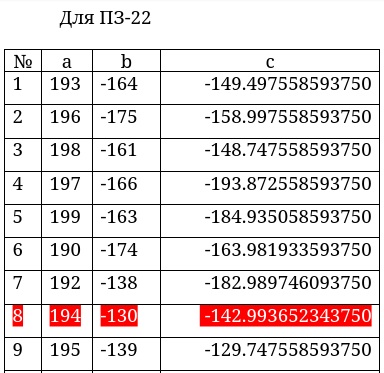
\includegraphics[scale=0.8]{v}
	\end{figure}

	\section*{Хід роботи}
	\section*{1.}
	\begin{Large}
		\begin{gather}
			194_{10} = 11000010_2 = 0000000011000010_2 = \boldsymbol{00C2_{16}}\nonumber
		\end{gather}
	\end{Large}

	\section*{2.}
	\begin{Large}
		\begin{gather}
			130_{10} = 0000000010000010_2\nonumber\\
			-130_{10} = 0000000010000010_2 \rightarrow 1111111101111101_2 \rightarrow 1111111101111110_2 =\nonumber\\
			= \boldsymbol{FF7E_{16}}\nonumber
		\end{gather}
	\end{Large}

	\section*{3.}
	\begin{Large}
		\begin{gather}
			0000000011000010_2+1111111101111110_2=\boldsymbol{0000000001000000_2}\nonumber
		\end{gather}
	\end{Large}

	\section*{4.}
	\begin{Large}
		\begin{gather}
			0000000001000000_2 = \boldsymbol{64_{10}}\nonumber
		\end{gather}
	\end{Large}

	\section*{5.}
	\begin{Large}
		\begin{gather}
			-142.993652343750_{10} \nonumber\\
			142_{10} = 10001110_2\nonumber\\
			0|993652343750\nonumber\\
			1|9873046875\nonumber\\
			1|974609375\nonumber\\
			1|94921875\nonumber\\
			1|8984375\nonumber\\
			1|796875\nonumber\\
			1|59375\nonumber\\
			1|1875\nonumber\\
			0|375\nonumber\\
			0|75\nonumber\\
			1|5\nonumber\\
			1|0\nonumber\\
			0.993652343750_{10} = 0.11111110011_2\nonumber\\
			142.993652343750_{10} = 10001110.011111110011_2\cdot2^{111} = 1.000111011111110011exp_{2^{111}}\nonumber\\
			E = 10000110_2\nonumber\\
			M = 00011101111111001100_2\nonumber\\
			-142.993652343750_{10} = \boldsymbol{11000011000011101111111001100_2} = \boldsymbol{0xC30EFE60_{16}}\nonumber
		\end{gather}
	\end{Large}

	\section*{6.}
	\begin{Large}
		\begin{gather}
			E = 10000000110_2\nonumber\\
			M = 00011101111111001100_2\nonumber\\
			-142.993652343750_{10} = \boldsymbol{11000000011000011101111111001100_2} = \nonumber\\ = \boldsymbol{C061DFCC00000000_{16}}\nonumber
		\end{gather}
	\end{Large}
	
	\section*{Висновки}
	Під час виконання розрахункової роботи я закріпив вміння переводити цілі додатні та від'ємні числа з десяткової в двійкову та шіснадцяткову систему числення, а також закріпив вміння переводити додатні та від'ємні числа з рухомою комою з десяткової в двійкову та шіснадцяткову систему числення.
	
\end{normalsize}
\end{document}
